\chapter{Vulkan}

\section{Intro}

\subsection{OpenGLBook Notes}

A graphics API is a software interface that allows the programmer to communicate
with graphics hardware.

In the 1980s the first dedicated graphics add-on cards also started to appear
which would pave the way for future developments by standardizing a
method of drawing computer graphics but didn't offer much in terms of graphics
capabilities.

Starting from he early 1990s computer games took a strong hold on the PC
platform and a real push for better looking and better performing real-time
graphics began.

Silicon Graphics (commonly referred to as SGI) was a company founded
in 1981 that specialized in 3D computer graphics and developed software and
hardware specifically for this purpose.
One software library that SGI developed was IRIS GL,
a library used for generating 2D and 3D graphics on SGI's high performance
workstations.
n the early 1990s, SGI was the market leader in 3D graphics workstations
because of their high performance hardware and easy to use software.

SGI cleaned up IRIS GL, removed all functionality that
did not relate to computer graphics and released it to the public in 1992 as
OpenGL, a cross-platform standardized API for real-
time computer graphics.

Software vendors would have to provide their own implementations of the
OpenGL standard on their platforms, and hardware vendors programs that
allowed OpenGL to talk to the underlying graphics hardware called "device
drivers"

OpenGL quickly became the industry leading real-time graphics API, as it
was basically the only one available on multiple platforms.

During the early 2000s, GPU performance grew exponentially as more soft-
ware features were moved to the GPU. The CPU became obsolete for rendering
real-time 3D graphics since it could not keep up with GPU developments. In
fact, the current method of rendering 3D graphics saw the CPU as such major
bottleneck that new methods had to be invented to circumvent its use.

In rendering real-time computer graphics, the software pipeline exists to
describe what we'd like to see on the screen. For example, if we'd like to display
a green square on the screen, computer software would describe with which
dimensions, color, and at which position of the screen to draw the square.
The software pipeline also provides access to functionality that draws the
geometry onto the screen. It is worth noting that the software pipeline does
not actually do any drawing or transformations, since on modern systems this
functionality is entirely implemented by the hardware.

\subsection{Learn WebGL}

In the early days, if programmers wanted to create computer graphics, they had to
write programs that directly talked to the graphics hardware.
As new hardware designs were created, the software had to be rewritten to
work with the new hardware.

\subsection{Graphics Book}

In the early days of computer graphics, if you wanted to draw an image on the
screen, you had to directly instruct the CPU to do so.
For example, drawing a line segment would require to run a loop and set the
color of each pixel lying along the line.
Because of this reason, graphics required a lot of CPU time.
Thus, graphics performance was very slow compared to today's standards.

Computers nowadays are obviously faster than back then.
But the big change is that in modern computers graphics processing is done
by a specialized component called a GPU, or graphics processing unit.
A GPU includes processors for doing graphics computations.
A GPU can include a large number of processors that work in parallel
to greatly speed up graphics operations.
GPUs also include their own dedicated memory.
GPU processors have very fast access to data directly stored on the GPU itself,
much faster than their access to data stored in RAM.

To draw a line or perform some other graphical operation, the CPU simply
has to send commands, along with any necessary data, to the GPU, which is
responsible for actually carrying out those commands. The CPU offloads most
of the graphical work to the GPU, which is optimized to carry out that work
very quickly. The set of commands that the GPU understands make up the API
of the GPU. OpenGL is an example of a graphics API, and most GPUs support
OpenGL in the sense that they can understand OpenGL commands, or at least
that OpenGL commands can efficiently be translated into commands that the
GPU can understand.

\subsection{History Of OpenGL}

The main goal of an API is to
abstract the underlying implementation of software and hardware and provide
the developer the tools to interact with them.
Graphics APIs are implemented
by driver software that is written by graphics hardware vendors specifically
for each hardware. They are the medium with which developers can control
the dedicated graphics hardware by issuing various implementation-agnostic,
higher-level commands to the software driver who in turn translates them to
lower level commands for each specific hardware.

The state of the art in graphics was
using software rendering. The best that could be achieved without hardware
acceleration was a small amount of simple colored, filled polygons.

As time passed, the prices of graphics hardware declined, and their performance
increased. Furthermore, new features were added to the now low-cost
graphics processors which in turn were added to the OpenGL specifications as
well.

Some of these extensions interacted well with each other and
with already existing feature of OpenGL and
some did not. Moreover, as newer ways of taking advantage of the GPU were
invented they were added in OpenGL as well, resulting in having multiple ways
available to do the same thing.

\subsection{Red Book}

In the early days of graphics programming, drawing images on the screen was very
slow.

In the late 1970s, a professor at Stanford (Jim Clark) had the idea to try
to build specialized hardware to do graphics (relatively) fast and fit it into a
workstation.
He and his students started a company to bring the machines to market. The
company was called Silicon Graphics (SGI).

In the mid- to late- 1990s, other companies realized that GL was a good
way to program graphics, and wanted to let programmers work that way. So, a
standards group was formed and they created OpenGL. OpenGL was designed
so that it didn't require SGIs hardware and operating system. But, it worked like
GL, which was designed with SGI's hardware in mind.

For a while, this was great. We had a convenient way to program graphics
that worked across different platforms. But then, graphics hardware evolved.
Very quickly. OpenGL had to be extended to provide people with access to
these new features.

While the old ways of programming graphics (i.e. what the SGI
hardware did in 1990) was convenient for many things, and was the most efficient
way to do stuff for circa 1990 computers, it was not at all how modern hardware
worked.

So, in the late 2000s, early 2010s, the folks in charge of OpenGL decided to
remove all of the old circa 1980s/1990s stuff designed for SGI hardware.

\section{What is Vulkan?}

\begin{wrapfigure}{l}{0.4\textwidth}
    \begin{center}
        
\includegraphics[scale=0.10]{images/ChVulkan/VulkanLogo.png}
    \end{center}
    \caption{Vulkan logo}
    \label{fig:VulkanLogo}
\end{wrapfigure}

Vulkan is a modern graphics API. It is maintained by the Khronos Group.
Vulkan is meant to abstract how modern GPUs work.
Using Vulkan, the programmer can write more performant code.
The better performance comes at the cost of having a more verbose and low level API compared to
other existing APIs such as OpenGL or Direct3D 11 and prior.
Vulkan is not the only modern graphics API, other such APIs are Direct3D 12 and Metal.
Nonetheless, Vulkan has the advantage of being fully cross platform.

\section{What problems does Vulkan solve?}

\begin{wrapfigure}{l}{0.4\textwidth}
    \begin{center}
        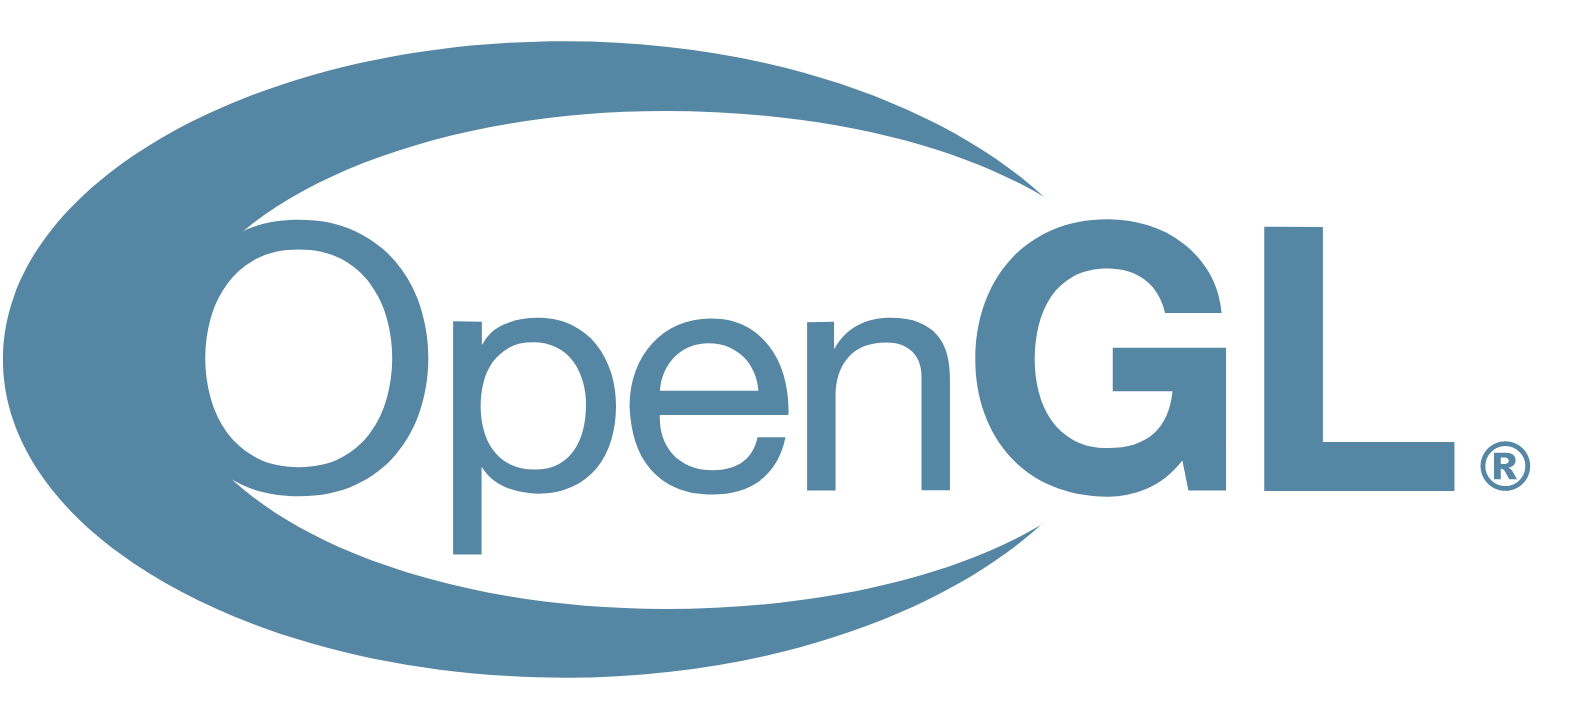
\includegraphics[scale=0.10]{images/ChVulkan/OpenGLLogo.png}
    \end{center}
    \caption{OpenGL logo}
    \label{fig:OpenGLLogo}
\end{wrapfigure}

Common graphics APIs like OpenGL or Direct3D were developed during the 1990s.
At that time, graphics card hardware was very limited not only in terms of computational
power but also from a functionality standpoint. As time progressed, graphics card architectures
continued to evolve, offering new functionalities.
All these new functionalities had to be integrated with the old existing APIs.
The more new functionalities were integrated, the more the GPU's driver complexity grew.
Such complicated GPU drivers are inefficient and are also the cause of many
inconsistencies between implementations of the same graphics API but on different GPUs.

\section{How does Vulkan solve these problems?}

Vulkan doesn't suffer from the problems we saw above because it has been designed from scratch
and with modern GPU's architecture in mind.
It reduces the driver overhead by being more verbose and low level.
It is also designed to be multithreaded, allowing the programmer to submit GPU commands from
different threads.
This is very beneficial to performance, since modern CPUs usually have more than one core.
